\documentclass[11pt]{article}
\usepackage[margin=0.85in]{geometry}
\usepackage{graphicx,booktabs,amsmath,hyperref,xcolor,microtype}
\usepackage[T1]{fontenc}
\usepackage{lmodern}
\definecolor{ink}{HTML}{17283D}
\definecolor{accent}{HTML}{087F8C}
\hypersetup{colorlinks=true,urlcolor=accent,linkcolor=accent,citecolor=accent}
\setlength{\parindent}{0pt}
\setlength{\parskip}{5pt}
\author{James Jean\\\small Independent research}
\date{28 October 2026\\\small GitHub research manuscript; not peer reviewed}

\title{\color{ink}Low acceleration error can hide missed deceleration\\[4pt]\large A road-transfer study with frozen model and alert selection}
\begin{document}\maketitle
\begin{abstract}
A fleet analyst considering a deceleration alert needs both a stable reference estimate and adequate event coverage. This study trains past-only speed-based estimators on I-80, selects among 18 candidates on Lankershim Boulevard and evaluates the frozen choice on US-101. A shallow gradient-boosting model achieves trajectory-balanced test RMSE of 0.291 m/s$^2$, compared with 1.417 for the validation-selected zero-acceleration baseline. Yet its conservative, validation-fixed alert threshold recalls only 23.7\% of strong reference-deceleration frames, with 99.7\% precision. Low reconstruction error therefore does not establish useful event coverage. The labels are processed NGSIM accelerations sharing provenance with the speed input, not independent braking ground truth; the result is an offline signal-reconstruction finding, not a safety validation.
\end{abstract}

\section{Question and prior evidence}
An alert can be statistically precise while missing much of the condition it is meant to identify. The operational question is whether a past-only estimate and a conservative operating point remain useful when the road environment changes. Selecting a model solely by regression loss cannot answer that question.

NGSIM trajectories have known measurement limitations. Montanino and Punzo document errors amplified by differentiation and propose reconstruction methods \cite{montanino}. Coifman and Li critically evaluate the underlying trajectory data \cite{coifman}. This study does not resolve those errors. Its narrower contribution is a reproducible cross-road comparison of a regression selection objective and an alert-coverage objective, with complete candidate evidence and an explicit reference-label limitation. No new learning algorithm or globally novel research gap is claimed.

\section{Data, rights and cohort}
The official FHWA/DOT source contains video-derived vehicle trajectories at 0.1-second intervals \cite{dot}. We retained vehicle IDs 1--80 at I-80, Lankershim and US-101: 81,147, 40,876 and 124,121 rows, respectively. All 246,144 downloaded rows reconcile to independent source-count queries, and six page hashes identify exact source bytes. This is a convenience cohort of early IDs, not a random or network-representative sample.

Anonymous IDs repeat across recording intervals. Tracks are therefore split on any time increment other than 100 milliseconds or frame increment other than one. Identical rows would be deduplicated and ambiguous vehicle/time keys rejected; neither occurred in this cohort. Removing the first ten history-incomplete frames of each segment leaves 80,237 training, 40,156 validation and 121,981 test frames, from 91, 72 and 214 tracks. No global coordinates, video, plates, faces or personal records are retained. Source excerpts and adaptations carry the source's CC BY-SA 3.0 terms.

Feet are converted to meters using exactly 0.3048. The target is recorded acceleration. Features are current speed; backward speed differences over 0.1, 0.3, 0.5 and 1.0 seconds; and mean and standard deviation over the ten preceding speed observations. SQL lag windows preserve explicit timestamps. No acceleration lag, future frame or centered smoother enters the model. Upstream source processing may itself use future information, so past-only feature construction does not establish live sensor availability.

\section{Optimization and evaluation}
I-80 is used only for fitting; Lankershim only for model and threshold selection; US-101 only for final evaluation after the selection artifact is frozen. There is no shuffled frame split or refitting with validation/test data. Each training trajectory receives equal total sample weight. Scaling for ridge is fitted on training data alone.

Five baselines comprise zero acceleration and four backward-difference windows. Ridge penalties are 0.01, 0.1, 1, 10 and 100. Eight histogram-boosting configurations cross depth 2/3, learning rate 0.05/0.1 and L2 0/1, with 100 iterations, minimum leaf size 30, early stopping disabled and seed 20261028. The primary objective is
\[
\mathrm{MSE}_{\mathrm{track}}=\frac1G\sum_{g=1}^{G}\frac1{n_g}\sum_{i\in g}(a_i-\hat a_i)^2,
\]
which gives each contiguous track equal influence. All 18 candidate scores and runtimes are retained. Raw frame-weighted errors are reported separately. A finite grid is not a global optimum; a single validation road does not characterize generalization across roads.

The selected model has depth 3, learning rate 0.05 and L2 zero. The selected baseline is zero acceleration. For each, thresholds from $-12$ to $-4$ feet/s$^2$ in steps of 0.5 maximize validation recall subject to at most 1\% frame-level false positives. Ties favor lower false-positive rate and then a more conservative threshold. The reference-positive rule is acceleration $\leq-8$ feet/s$^2$ ($-2.4384$ m/s$^2$), an analytical choice rather than a regulatory safety definition. The boosting alert threshold is fixed at $-3.2004$ m/s$^2$ before test scoring.

\section{Results}
Trajectory-balanced MSE on the held-out road is 0.0846 m$^2$/s$^4$ for boosting and 2.0068 for the baseline. Their paired difference is -1.9222, with a 95\% trajectory-resampling interval of [-1.9866, -1.8624], using 2,000 draws. This interval is conditional on the sampled road and assumes resampled tracks are independent; shared traffic conditions weaken that assumption.

\begin{table}[ht]\centering
\caption{Frozen boosting alert on 121,981 US-101 frames. Counts concern processed reference acceleration, not independently observed brake use.}
\begin{tabular}{lr}\toprule
Measure & Result\\\midrule
True positives & 1,614\\
False positives & 5\\
Missed reference positives & 5,187\\
True negatives & 115,175\\
Precision & 99.7\%\\
Recall & 23.7\%\\
False-positive rate & 0.0043\%\\
\bottomrule\end{tabular}\end{table}

The constraint is satisfied on this test road, but most reference positives are missed. The zero baseline issues no alerts and has zero recall; its precision is undefined. A model can therefore improve the declared regression objective without making the resulting conservative alert an adequate screening system. Threshold relaxation is a hypothesis for a new evaluation, not a post-test change made here.

\begin{figure}[ht]\centering
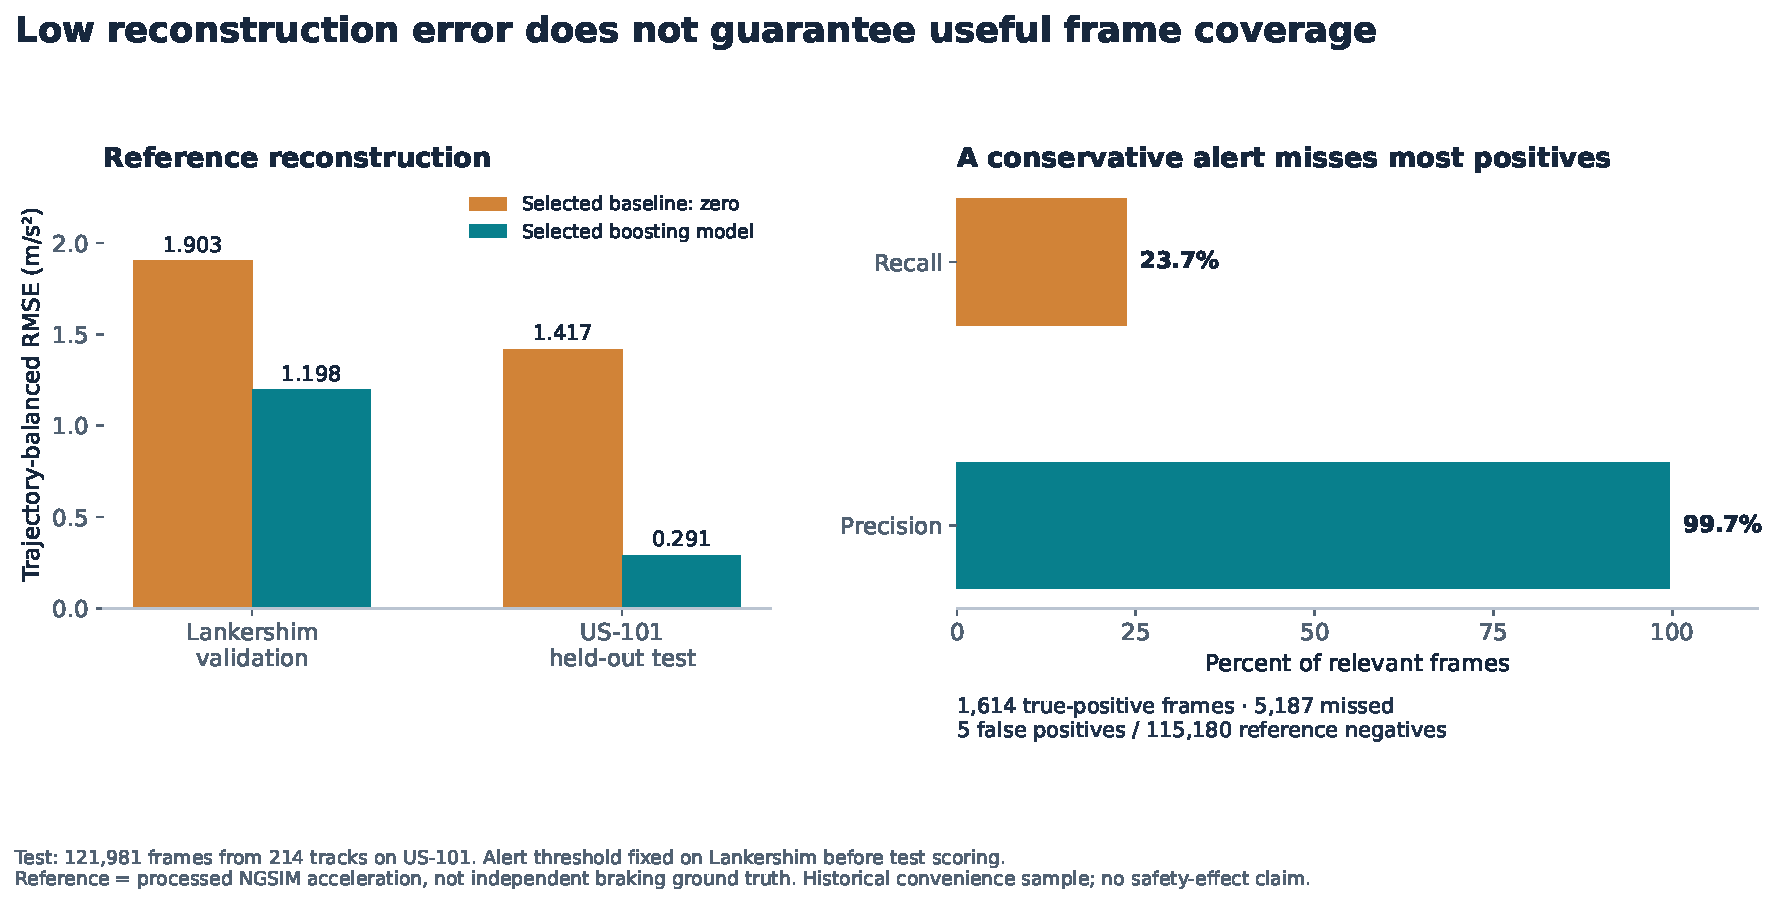
\includegraphics[width=\linewidth]{images/decision-summary.pdf}
\caption{Regression performance and alert usefulness must be assessed separately.}
\end{figure}

\section{Checks, limits and next decision}
An independent verifier recomputes every source join, metric, candidate selection, threshold confusion count and paired interval from exports without importing the fitting implementation. It caught a cancellation error in the standard-deviation calculation at constant speed. Centering each short window repaired the arithmetic before the final test; the original failed check and selection record are retained. The repair did not change the protocol or inspect test outcomes.

The main limitation is shared provenance between input speed and processed reference acceleration. Low MSE cannot validate a sensor or brake-event detector against independent truth. The cohort is small in roads, historically dated and selected by ID; adjacent frames and different vehicles share conditions. Track resampling does not resolve those dependencies. Frame-level recall is not event-level detection latency. Vehicle-class and speed-group diagnostics are descriptive and do not alter the selected model.

The practical recommendation is to evaluate independently instrumented acceleration and brake actuation on additional roads before operational use. Define an acceptable miss rate with the intended user, retain an untouched route cohort and test the threshold there. This study supports that evaluation design, not deployment, regulatory compliance or measured safety gains.

\section*{Reproducibility and authorship}
Public code, licensed source excerpts, frozen selection, all candidate predictions, independent checks and figures are at \url{https://github.com/S3R3Bii/brake-signal-transfer}. This research manuscript is shared with the reproducible GitHub package and has not been peer reviewed. The work used AI-assisted coding and drafting. Executed results are distinguished from proposed follow-up work.

\begin{thebibliography}{9}
\bibitem{dot} Federal Highway Administration. \emph{Next Generation Simulation Vehicle Trajectories and Supporting Data}. U.S. DOT, dataset 8ect-6jqj. Accessed 28 October 2026. \url{https://data.transportation.gov/api/views/8ect-6jqj.json}.
\bibitem{montanino} M. Montanino and V. Punzo. Making NGSIM Data Usable for Studies on Traffic Flow Theory: Multistep Method for Vehicle Trajectory Reconstruction. \emph{Transportation Research Record}, 2390, 2013. \url{https://doi.org/10.3141/2390-11}.
\bibitem{coifman} B. Coifman and L. Li. A critical evaluation of the Next Generation Simulation (NGSIM) vehicle trajectory dataset. \emph{Transportation Research Part B}, 2017. \url{https://ceg.osu.edu/sites/default/files/2022-06/Coifman_and_Li_2017.pdf}.
\end{thebibliography}\end{document}
